%!TEX root = ../thesis.tex
%*******************************************************************************
%****************************** Third Chapter *********************************
%*******************************************************************************

\chapter{Reductions in Orangutan Flange Size after Initial Development: Relationship to FAI, Antagonistic Interactions, and Age}

Male orangutans are bimature with two sexually active male morphs: the unflanged male and the flanged male. Unflanged males are similar to females in overall appearance, whereas flanged males have a larger body mass, more hair, developed throat sacs capable of making long calls, and large fatty cheek pads known as flanges. Numerous field sites have anecdotally reported the presence of flanged males with degraded flanges, which in some research has been associated with the term "past-prime". I investigated 3 potential causes of this condition by measuring flange size after initial development at two sites across multiple photographs of the same individuals and correlated these observed changes with local FAI, antagonistic interactions, and behavioural data to examine the cause of this condition. In addition, I explored the relationship between changes in individual flange size with long calls, copulations, and female association. I found that flange size deterioration is driven by age, and individuals with diminished flanges produce more long calls per day. This research suggests that maintenance of the flange size is not metabolically costly and that variance in flange size after development is likely not due to ketosis, but may be driven by age-related deterioration of muscle fibres and connective tissue that supports the structure of the flange.

\section{Introduction}
Sexual selection provides an important theoretical framework for understanding the role that inter-sexual mate choice and intra-sexual competition play on the evolution of traits, behaviours, and ecology. While in theory inter-sexual selection and intra-sexual selection apply to both sexes, in mammals due to anisogamy precopulatory intra-sexual selection typically has more impact on male-male competition, and inter-sexual selection primarily reflects female mate choice \citep{Andersson.1996}. However, how sexual selection applies to specific species must be viewed under the lens of which mating system the species has, as each mating system has associated strategies to maximise fitness \citep{Kappeler.2004}. For example, in polygynandrous mating systems, males often employ many post-copulatory evolutionary strategies to maximise the chances of successful fertilisation, including particularly adaptations to the testes and penis \citep{Ros-Santaella.2015}. For example, male mandrills have large testes in relation to their body size that increase in volume up to 25\% during the mating season \citep{Setchell.2001}. Additionally, their sperm coagulates after insemination, forming a plug that increases the chances of the individual to fertilise by decreasing the opportunities of the other for successful insemination \citep{Setchell.2016}. Similar adaptations are observed in chimpanzees, which also have large testes relative to their body weight, more than 16x larger than gorilla testes relative to their body weight \citep{Dixsonwr}. These adaptions reflect species maximising fertilisation rates under social systems where the number of matings for both sexes is less limited. However, where the number of matings is limited, sexual selection acts primarily on pre-copulatory behaviour \citep{Andersson.1996, Cassini.2020}. Therefore, to increase reproductive fitness, individuals develop strategies based on the location, attraction, and monopolisation of access to mates, and these strategies often utilise secondary sexual characteristics \citep{Kappeler.2004}. 

Secondary sexual characteristics (SSCs)  can take the form of weapons that can be used to fight for access to mates, and ornaments that are otherwise non-functional traits used to signal fitness to receptive females and to signal relative dominance to other males to prevent costly antagonistic interactions \citep{Kappeler.2004}. To be honest indicators of fitness, SSCs are energetically costly and usually an active hindrance to the survival of the individual \citep{Zahavi.1975}. Despite these high costs, the signal poses significant benefits to the signaller and receiver: for males, producing high-quality SSCs is a trade-off between maximising lifespan vs. number of matings, where a significantly reduced lifespan is a worthy trade-off for a significant increase in the number of copulations \citep{Petersen.2020b6j}. Providing the SSCs are honest fitness indicators, selective females are then able to choose mates with greater than average fitness, which can then be passed onto their offspring. These female preferences for mates with high-quality SSCs allow both the SSCs and the preference to be maintained in the population through directional selection \citep{Gomulkiewicz.1991}. 

In species that possess them, producing high quality SSCs is paramount for reproductive success, however, it is important to note that these signals only impact pre-copulatory sexual selection, and the relationships between SSCs and \textit{post}-copulatory mating success vary depending on species, and there are few universalities \citep{Setchell.2003}.  

In general, there appears to be an energetic trade-off to be made with investing in ornaments used to attract mates and relative testes size, \textit{i.e.} between pre and post copulatory mating strategies, as there is an observed negative correlation in most primates between SSC ornament size and testes size \citep{Lüpold.2019}. The theory being that a large investment in secondary sexual ornaments increases the chance of female monopolisation, there is less sperm competition and hence less of a need to invest in testes size \citep{Simmons.2017}; however, this hypothesis has a couple of flaws. Firstly, this trend is not universal and in some species high-quality ornamental SSCs are positively correlated with testes size. For example, in probosis monkeys, a study of 18 males found that nose size was positively correlated with testes size, suggesting that in some species testosterone may be a functional link between expressed SSCs and post-copulatory fitness \citep{Matsuda.2020g6t}.  Secondly, across primates there appears to be a positive correlation between canine size (which can be used as sexual ornaments) and testes size, which is contrary to the theoretical negative relationship between ornaments and testes size \citep{Lüpold.2019}. 

However, the reason for this seeming contradiction may be due to the practicalities of monopolising access to mates. While the best way to maximise fitness under sexual selection theory is to monopolise access to multiple females,  when this is not possible, the next best strategy is to maximise the number of copulations \citep{Setchell.2016}. Weapons have the advantage of being used as indicators of fitness during male-male competition and to be used for coercive mating. Furthermore, purely ornamental signals of fitness are generally metabolically costly to maintain, as well as to produce; while canines are metabolically costly to produce, their metabolic maintenance may be significantly lower or use different resources to maintain compared to SSC ornaments \citep{Lüpold.2019}. 

\subsection{Testosterone, cortisol, hierarchy stability and dominance}

In diverse primate taxa, testosterone plays a crucial role in the development and maintenance of male secondary sexual characteristics (SSCs), with variations in the hormone's effects observed across species. Chimpanzees, for example, show a robust correlation between elevated testosterone levels and the manifestation of SSCs such as larger body size, and increased dominance \citep{Dixson}. Likewise, mountain gorillas display notable differences in testosterone levels between dominant silverback males and subordinate males \citep{Robbins.2004}, with silverbacks developing significant muscle mass, larger body size, and distinctive silver hair. Long-tailed macaques present another example, where dominant males with higher testosterone levels exhibit well-developed canine teeth and increased aggression during mating season \citep{Girard-Buttoz.2014}.

To better understand the role of testosterone in SSC development, it is essential to consider the challenge hypothesis. This hypothesis posits that testosterone levels in male animals are tightly regulated, primarily increasing in response to social challenges such as male-male competition, territorial disputes, and mate guarding \citep{Wingfield.1990}. According to this hypothesis, testosterone levels should rise during periods of social instability or competition and decrease during social stability when the costs of high testosterone outweigh the benefits. The challenge hypothesis specifically contends that variations in testosterone levels during the breeding season correlate more closely with male aggression in reproductive contexts than with changes in reproductive physiology \citep{Wingfield.2020}. Therefore, assessing the influence of testosterone on the development of SSCs requires acknowledging additional factors, such as species-specific social structures, mating systems, and ecological pressures, which also modulate the expression of these traits and their relationship with testosterone levels.

In some primates, circulating testosterone levels are directly influenced by the dominance of the individual within their social hierarchy, rather than being a predictor of future dominance. Basal testosterone and cortisol levels in individually housed cynomolgus monkeys (\textit{Macaca fascicularis}) did not predict eventual social rank, however, cortisol levels after social housing could predict whether an individual would become subordinate and basal testosterone levels were higher in dominant males \citep{Czoty.2009}. In bearded capuchins, alpha males have higher levels of circulating testosterone than their peers, even under unstable dominance hierarchies \citep{Mendonça-Furtado.2014}. Similar relationships can be seen in great apes.  In chimpanzees, even when controlling for age, circulating testosterone is positively correlated with both dominance rank and aggression rates against other individuals \citep{Anestis.2006}. But this pattern is not universal, in bonobos there is no correlation between dominance rank and testosterone levels in either sex \citep{Sannen.2003}. This divergence in the role of testosterone in these closely related species can be attributed to their different social structures and mating systems, and cautions overly simplistic interpretations of the causative role of testosterone on dominance or mating success.

Cortisol also plays a significant role in dominance in several primates. In some species, high-ranking individuals exhibit elevated cortisol levels due to the increased stress associated with maintaining their dominant status and engaging in aggressive interactions. In male chimpanzees, dominant individuals have been found to exhibit higher levels of cortisol compared to subordinates, particularly in situations of social instability and increased competition \citep{Muller.2004}. Similarly, in rhesus macaques, dominant males have been reported to display elevated cortisol levels, which has been associated with the increased frequency of agonistic encounters and the necessity of maintaining dominance rank \citep{Sapolsky.1992}. In contrast, other primate species demonstrate an inverse relationship between dominance rank and cortisol levels, with subordinate individuals exhibiting higher cortisol levels due to stress induced by their lower social status. For example, in Assamese macaques, subordinate males have been observed to display elevated cortisol levels, which has been linked to increased harassment and social subjugation experienced by these individuals \citep{Ostner.2008}. Furthermore, some primate species show more complex relationships between cortisol levels and dominance rank, wherein the association is influenced by factors such as social stability and group dynamics. For instance, in olive baboons, dominant males have been found to exhibit higher cortisol levels during periods of social instability, while subordinate males display elevated cortisol levels under stable social conditions \citep{Gesquiere.2011}. Generally, dominant males are predicted to undergo more stress under unstable dominance hierarchies than subordinant males, while the opposite is predicted under stable dominance \citep{Kappeler.2004}. However, in practice these predictions vary according to species, reflecting the diversity of the primate family. 

Regardless of the dominance system, the normal impacts of psycho-stress on individuals is usually a temporary condition as a result of an acute event, which leads to increases in cortisol and epinephrine \citep{Edes.2017}. These effects return to normal when the cause of the stress is removed, however under continuous social stress such as the stress of dominant male in a unstable dominance hierarchy this can lead to impacts on long term health \citep{Maestripieri.2011}. The cumulative effect of stress on health outcomes and disease is known as allostatic load, and these impacts are just starting to be examined in captive primates. In captive zoo-housed lemurs, smaller groups sizes, frequent group changes and cumulative time spent indoors all correlated with increased allostatic load \citep{Seeley.2021gr8}. In captive African great apes, age is significantly correlated with increased allostatic load; and notably in captive chimpanzees and western lowland gorillas, cumulative stressful events are also correlated with increased allostatic load \citep{Edes.2016,Edes.2023}. While the nature of the relationship between an individuals allostatic load and degradation of SSCs has not yet been explored in great apes, if SSCs are unbiased indicators of fitness elevated, presence of these biomarkers may be part of the mechanism that leads to degradation of the quality of the signal produced by the trait.


\subsection{Sexual selection and orangutans}

Orangutans are the only great apes to live outside of Africa \citep{Wich.2008}. Now only located in Sumatra and Borneo, they live in tropical forests characterised by their large variability in fruit production. Uniquely among great apes, male orangutans are bimature, meaning there are two sexually active male morphs: the unflanged male and the flanged male \citep{Prasetyo.2021}. Unflanged males are similar to females in body size and overall appearance, while flanged males have a larger body mass, more hair, developed throat sacs capable of making long calls and large fatty cheek pads, known as flanges \citep{Knott.2008}. Due to their semi-solitary social system and consequential difficulties in gathering large behavioural data sets, it's unclear whether orangutan SSCs are unbiased indicators of fitness, or even whether they all reflect the same measure of fitness. 

Male orangutans experience intense sexual selection, especially male-male competition and female choice. While flanged males are broadly tolerant of unflanged males, and unflanged males are largely tolerant of each other; interactions between two flanged males, while rare, are invariably antagonistic, and often result in significant injuries such as fingers or upper lip being bitten off \citep{Setia.2008}. Given that females do not advertise ovulation, have long inter-birth intervals, and the species' semi-solitary social structure, these factors are predicted to increase the intensity of male-male competition and suggest that monopolisation of females is the best strategy for maximising the number of offspring \citep{Galdikas.1985, Kappeler.2022}. However, interestingly in practice, aggression between flanged males appears to decrease in the presence of a female, suggesting that aggression rates may be due to highly overlapping ranges, as opposed to access to females \citep{Dunkel.2013,Marty.2015}.

Female orangutans show a strong mate preference for flanged males, resulting in the two morphs developing alternate mating strategies. Flanged males utilise a "call and wait" strategy, as their developed throat sacs enable flanged males to produce long calls, distinct vocalisations that travel up to 1.3km in the forest depending on the terrain \citep{Spillmann.2016}. Other flanged males do not significantly approach or move away from these calls, and unflanged males retreat; while females move towards the source of the call \citep{Setia.2007}. These calls have dual purposes: attracting females and acting as a spacing mechanism for flanged males \citep{Spillmann.2010}. When females do arrive, flanged males can enter consortships with them (which is more common during masting events), where they travel and nest together for a few days while sporadically mating \citep{Atmoko.2008saj}. 

Unflanged males, lacking the ability to make long calls, instead utilise a "silent searching" strategy: roaming around the forest in active search for females, and when they find them often resort to forced copulation, which is uncommon among great apes \citep{Atmoko.2008saj, Utami.2002km8}. 

Among flanged males, the most successful mating strategy varies depending on location. For example, Suaq Balimbing in Sumatra due to its high primary productivity and year-round fruit availability is capable of supporting the highest density of wild orangutans in the world, and these ecological factors support local dominant male and stable dominance hierarchies. However, in Tuanan, a site in central Kalimantan, where fruit and food availability is much more variable and hence ranges are larger, the social structure has a much more unstable dominance hierarchy, and some flanged males do employ the "search and find" mating strategy \citep{Kunz.2023}. Hence, the evolutionary stable strategy for male individuals depends on the level of monopolisation of females, and consequently sites with higher levels of monopolisation have a higher ratio of unflanged males to flanged males.

\subsection{Flanges and orangutans}

Flanges are the most conspicuous SSC that male orangutans develop. Physiologically, they are primarily formed of fat deposits bound to fibro-fatty tissues \citep{Straus.1942}. The initial growth of flanges begins with the other SSCs during the bimaturism process, which usually completes within 3 years, however during bimaturism antagonistic interactions from flanged males causes social stress which has been shown in some cases to arrest the bimaturism process \citep{Prasetyo.2021}. The exact trigger for bimaturism is unknown, however it is known that the triggering is not linked to nutritional availability, as individuals under nutritional stress can still go through bimaturism \citep{Prasetyo.2021}. There appears to be social correlates of the triggering of bimaturism, as the same social stresses that can arrest the growth of SSCs also appear to inhibit their development \citep{Dunkel.2013xnm}. These findings help explain the varying rates of bimaturism between sites and species. 

Overall flange size, shape and symmetry varies between individuals, sites and species, however their reflection of dominance relative to other flanged males, and indication of overall fitness is unknown \citep{Prasetyo.2021, Wich.2019}. There are observations from field stations in Borneo and Sumatra that have noted a reduction in flange size after their development \citep{Knott.2009b, Dunkel.2013}. This gives the flanges a shrivelled or deflated appearance. \citet{Knott.2009b} asserts the wider presence of a "past-prime" orangutan condition, with severely shriveled flanges which are subordinate to flanged males. 
Previous hypotheses have suggested that this may be associated with old age or nutritional deficiency, however any investigations into the cause of this condition have not yet been published \citep{Galdikas.1978,Knott.2008}. Nor has there been an attempt so far to quantify the magnitude of these changes.

As of yet, it remains unknown whether this condition is a physiological change that comes about after an individual has met a threshold condition, or whether there is larger variation in orangutan flange size after initial growth along a continuous spectrum. Given the physiology of the flange, and the metabolically costly nature of secondary sexual characteristics, maintaining a consistent size of these cheek pads may become compromised under specific environmental or individual conditions. A few possibilities as to the cause of this condition are:

\subsubsection{Nutritional deficiency as a cause of the "past-prime" condition}
Nutritional deficiency is a possible cause of this condition as orangutans live in forests characterized by irregularity and unpredictability in fruit production \citep{Morrogh-Bernard.2011}. Fruit production peaks approximately every 4 years in Sumatra during masting events triggered in part by the El Niño-Southern Oscillation phenomenon \citep{Wich.2000}. However when fruit is scarce, orangutans have been documented to have greatly reduced energy intake and fall into negative energy balance \citep{Erb.2018}. While fruit provides significantly greater energetic returns than fallback foods such as bark or pith, orangutans appear to have developed physiological adaptations to buffer against negative energy balance. Evidence of ketosis in wild orangutans is only seen during periods of low fruit availability, suggesting efficient energy storage as fat during periods of high fruit availability \citep{Erb.2018, Knott.1998}. 

However, for their body mass flanged males consume less calories than unflanged males, which may be due to unflanged males showing increased roving behaviour compared to the flanged male \citep{Vogel.2017}. Given that flanges morphologically are primarily adipose tissue, under ketosis this adipose may be burned for additional energy. Hence under this hypothesis, the flange serves as an honest signal of energetic balance for the purposes of mating, and the ability of the signaller to buffer against environmental change. 

\subsubsection{Antagonistic social stress}
However the social stresses that arrest and inhibit development may also be the cause of this condition. Antagonistic interactions have been shown to spike cortisol levels, which are correlated with inhibited flange development \citep{Thompson.2012}. These interactions can be indirect, as in both unflanged males and flanged males, hearing another flanged males long call causes an increase in cortisol levels \citep{Prasetyo.2021}. Both of these causes are somewhat secondary, and trigger activation of hormonal pathways for development of flanges and other associated SSCs. The understanding of the hormonal processes driving bimaturism are murky due to the semi-solitary social structure of orangutans, as well as their arboreal lifestyle making measurement difficult. Current evidence is inconclusive, however it does appear that testosterone is correlated with delayed flange development in captive orangutans \citep{Thompson.2012, Muller.2017}. However, captive orangutans' hormonal profiles are significantly different to wild populations, for example captive populations experience significantly higher levels of cortisol, and reduced levels of testosterone \citep{Prasetyo.2021}. However the same hormonal processes that drive initial flange development, may also impact the maintenance of these SSCs, and in turn interact with some of the other potential causes, as it's been noted that variation in feeding rates appears to drive differences in cortisol levels in some field sites \citep{Prasetyo.2021}.

\subsubsection{Relative age}
In polygynous and polygynandrous species, senescence is experienced more severely by males compared to females, due to a combination of evolutionary and early life factors \citep{Graves.2007}. Species with high levels on intra-sexual competition have a higher risk of mortality, which can lead to a reduction in the selection against deleterious mutations which can impact senescence \citep{Williams.1957}. However these factors are complicated by individual history of the individual, as early life adversity can impact the onset and severity of senescence \citep{Beirne.2015} Additionally, age may act as a synergistic factor which increases the impact of ecological stressors on individuals. Older individuals may have more difficulty accessing or processing food sources, which may in turn impact their health over time. Previous research has indicated correlations between maintained low dominance ranking and chronic psycho-social stress in rhesus macaques \citep{Maestripieri.2011}. These impacts then cause an allostatic load on the individual which can increase the probability of age related cognitive decline, mortality risk and cardiovascular disease. These results indicate a synergistic interaction between age and antagonistic interactions, however social stress in primates depends heavily on the stability of the dominance hierarchies of the chosen species and habitats \citep{Czoty.2009, Mendonça-Furtado.2014, Muller.2004}. 


\subsubsection{Correlations with long call behaviour}
If one of the aforementioned factors does correlate with a decrease in overall flange size, then the same metabolic pathways that impact flange size may have impacts on other associated SSCs. Male orangutans develop their complex throat pouches during bimaturism, and development can be arrested in the same way that flange development via the same psychoendoneurological mechanisms \citep{Prasetyo.2021}. Long calls contain contextual clues about the individual producing them and is the first way females are able to assess the quality of flanged males \citep{Spillmann.2010}. These calls can be made spontaneously or in reaction to hearing another long call as a method of confrontational assessment \citep{Spillmann.2016}. While previous studies have not seen a relationship between fruit availability and long call rates (suggesting they are not energetically costly to produce), individual body condition may still impact the duration or composition of long calls during periods of low fruit availability \citep{Spillmann.2016}. Additionally, age related muscle deterioration may reduce the the duration or number of pulses in a long call.

\subsubsection{Impacts on mating behaviour}
If relative flange quality is a SSC used to discern mate choice, then we would expect individuals with a reduction in overall flange size to experience negative outcomes when associating with females. In particular, females will either reduce the time spent in association with these flanged males during fertile periods, or reduce time spent in association with them altogether. Additionally, as females will not willingly copulate with individuals of poor quality we would expect to see either a reduction in overall copulation rates per hour of female association or an increase in the proportion of copulations that are forced.

\subsection{Study Aims}
This study aims to investigate the underlying causes impacting the observed variation in orangutan flange sizes and shapes after their initial development, and what life history or ecological factors are correlated with these changes. Additionally I wish to explore correlations between a change in flange size with long call rates, composition and duration; as well as impacts on mating success. 

Given the different ratios of flanged males to unflanged males/females between sites, the adipose content of flanges and the differing ecologies of the two sites, I predict:

\begin{enumerate}
    \item   Temporary reduction in flange size, where present, will follow periods of significant decreases in fruit availability.
    \item Antagonistic male-male interactions, including fights, will also cause flange size reduction due to the psychoendocrinilogical stress of the interaction.
    \item As decreases in overall fruit availability will lead to increases in ranging behaviour, rates of male-male interaction will also increase; causing an interactive effect between these ecological and social factors.
    \item Due to ecological and population differences between sites, I predict these effects will be seen more commonly in Tuanan compared to Suaq Balimbing.
    \item Individuals experiencing temporary reduction in flange size will produce long calls less often, or for a short period of time with fewer pulses.
    \item Individuals experiencing temporary reduction in flange size will spend fewer hours per follow day in association with females, and will have fewer proceptive copulations.
\end{enumerate}

\section{Methods}
\subsection{Study sites}
Data was collected at two field sites of high orangutan population density: Suaq Balimbing (located in Sumatra) and Tuanan (located in Borneo).

Suaq Balimbing Research Station (3°04'N, 97°26'E) is a field site located in the Gunung Leuser National Park  in south Aceh, Sumatra. Suaq Balimbing is a primary peat-swamp forest, which contains the highest density of wild orangutans in the world, with approximately 7.0 individuals/ km$^{2}$, supported by the availability of fruits year-round and comparative lack of anthropogenic disturbance \citep{Fox.2004, Schaik.1995}.

Tuanan Orangutan Research Project (2°09'S, 114°26'E) is located in the Mawas Reserve in Central Kalimantan, Borneo. Tuanan Research Station is located in a section of peat-swamp forest, and contains approximately 4.5 individuals/km$^{2}$, and the density of orangutans is among the highest in Borneo \citep{Husson.2008} . The site has a history of anthropogenic disturbance, including selective logging, and is increasingly suceptible to wild fires \citep{Cochrane.1999, Erb.2018}.

\subsection{Flange data}
Individuals were described as flanged, flanging or unflanged depending on their physical appearance. While the exact flanging onset remained ambiguous (as some large unflanged males might display minor cheek protrusions for multiple years due to the differential impact of socially induced development arrest) \citep{Kunz.2023}, the transition between the unflanged and flanged states was markedly distinct. Flanged males have fully developed SSCs and are capable of making long calls. Behavioural and photographic data was only used by individuals coded as "flanged".

Photographs were taken opportunistically during behavioural follows, including of associated party members. In this study due to the strict photographic requirements, all photographs were taken during focal follows of the individual studied. Since it was not possible to obtain pictures of orangutans from a fixed distance, flange size measurements taken are relative to the distance between facial landmarks (LMs) (see Chapter 2). Photographs were chosen where the orangutan is facing the camera head on, and were discarded if they were blurry, poor resolution or if any of the LMs could not be accurately placed. 

The photographs were orientated such that the middle of each pupil fell on a horizontal line, and 6 facial LMs were placed on the orangutans face. For detailed explanation of how these LMs were recorded, see Chapter 2. Two measures of orangutan flange size were used for this study.  

\begin{figure}
    \centering
    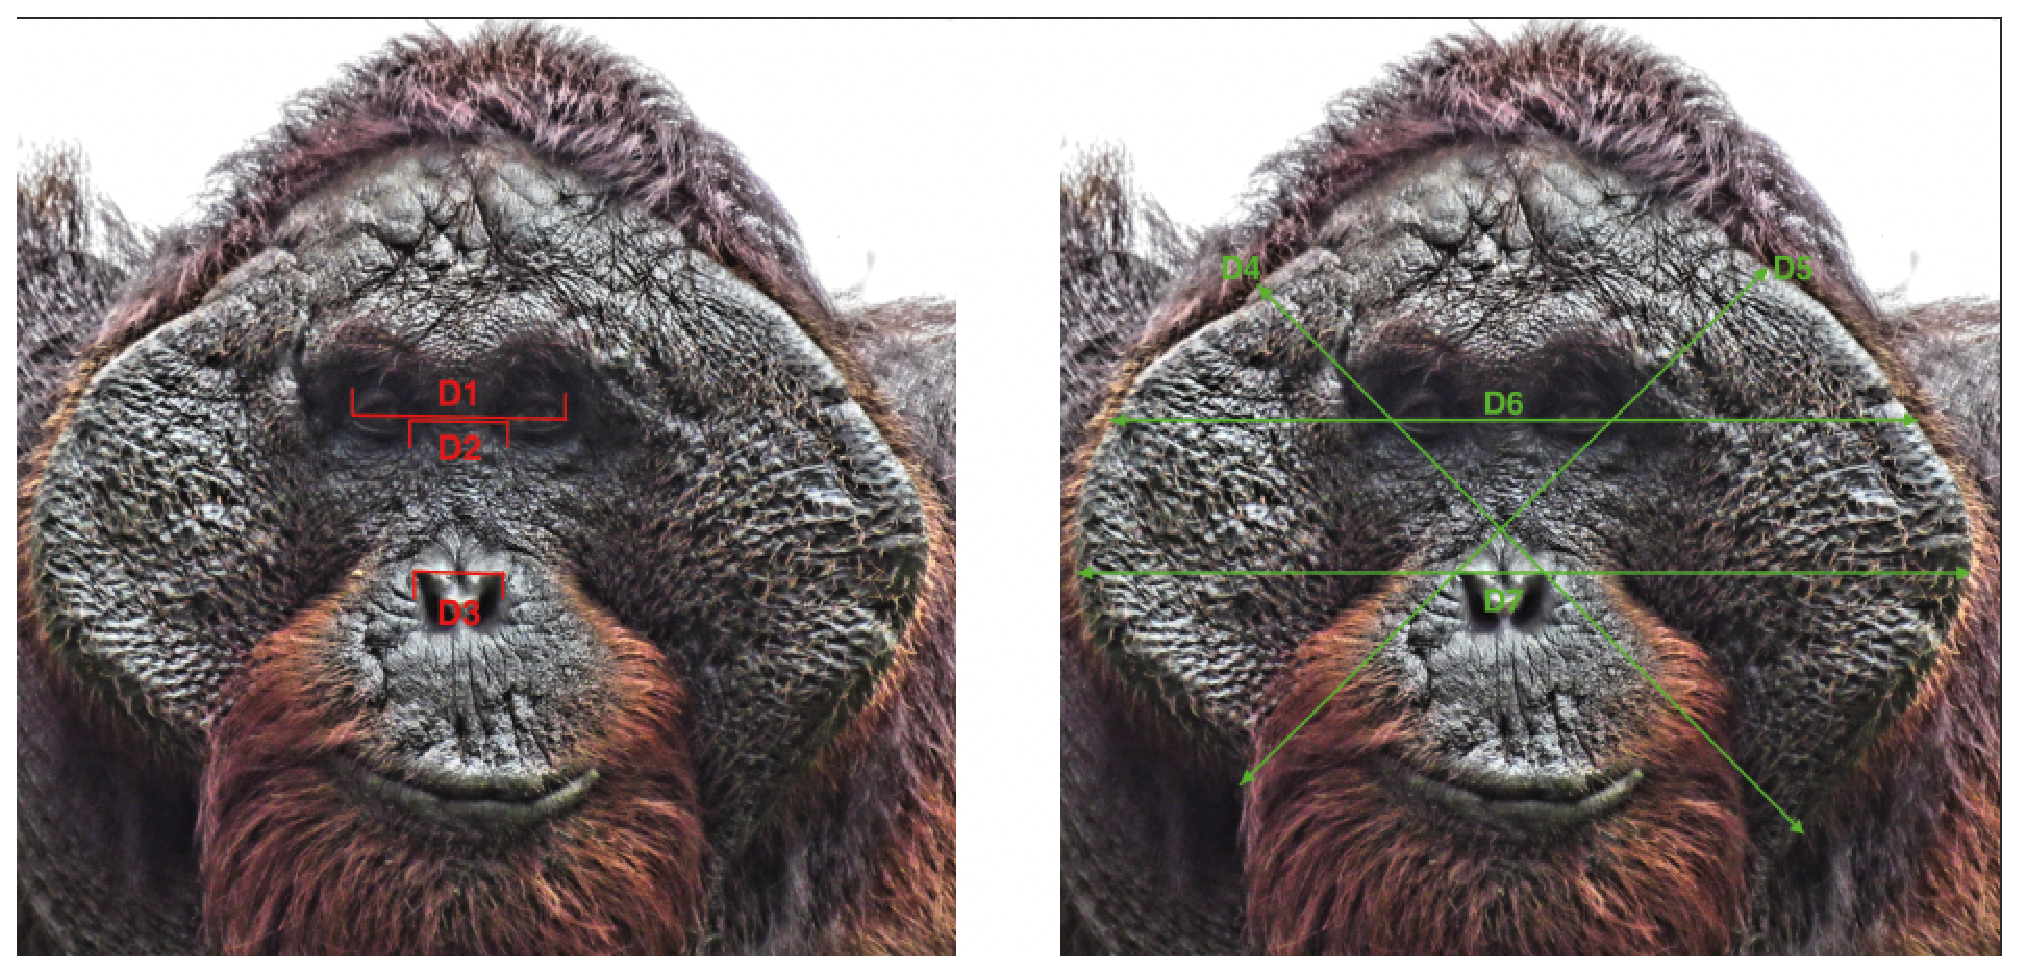
\includegraphics[width=1.0\textwidth]{Chapter3/Figs/mawasboth.eps}
    \caption{Facial LM placement on an example flanged male. Left image a) Relative flange width was estimated for each individual on a given follow day as \(  \frac{D6 \div D2}{D6\textit{max} \div D2\textit{max}}\) . Right image b) Relative flange area was calculated as the area contained within the irregular shape bounded by the points P\textit{n} using Gauss's formula}
    \label{fig:orangutanfameasures}
\end{figure}

The relative width of the flange was estimated by placing LMs on the inner tips of the eyes of each photograph and drawing a horizontal line to connect the two LMs (Figure 3.1.) This line was then extended until it reached the edge of the flange. The length (pixels) of the connecting line was divided by the inner eye distance to provide a relative measurement of flange width. To obtain comparable measurements, the relative flange width measurement was divided by the maximum recorded flange width measurement for each individual, so that each photograph has a proportional measurement of flange width between 0 and 1. Individuals with only one suitable photograph were not used for statistical analysis. This measurement of flange width was chosen due to its reliability during measurement and because of the intersection of the \textit{Mm. orbitotemporalis}, \textit{Mm. frontalis}, and \textit{Mm. zygomaticus} muscles around the eye and the high content of adipose tissue, this is the area hypothesised to be under the most pressure from my hypothesised causes \citep{Winkler.1989}. 

Relative flange area was estimated by placing 8 LMs on the orangutan's flanges by bisecting facial LMs as shown in Figure 3.2.  The area of the irregular shape enclosed by these coordinates was calculated using Gauss's area formula. This area was then divided by the square of the inner eye distance to provide a relative measure of flange area. Comparable measurements were obtained using the same method as for flange width, by dividing each image's relative flange area by the maximum recorded value for that individual. Images were rejected if they did not contain all 8 flange LMs. 

\begin{figure}
\centering
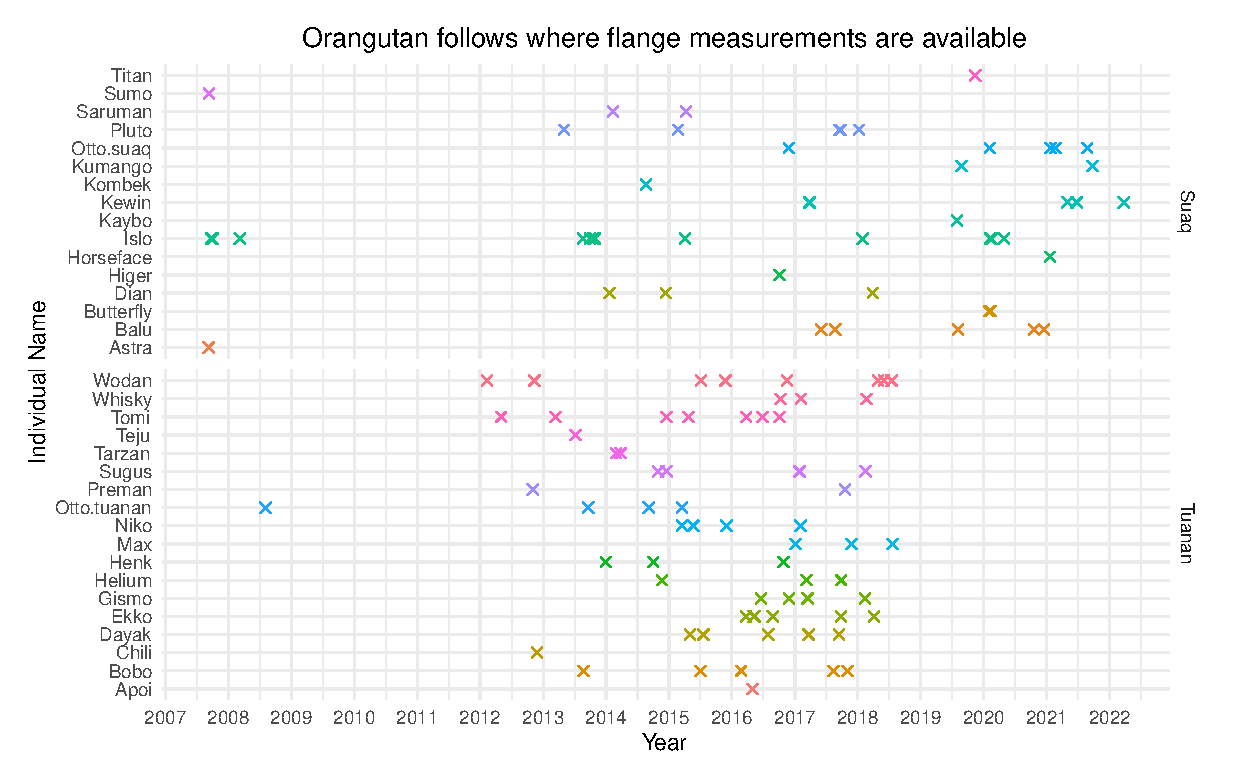
\includegraphics[width=1\linewidth]{Chapter3/Figs/sightings_plot.eps}
\caption{Timeline (x-axis) illustrating days where a flanged male was followed (ie focal individual), and the resulting photgraphs were of sufficient quality to obtain relative flange measurements at Suaq Balimbing and Tuanan. Individuals with only one suitable photograph were not used for analysis.}
\label{fig:orangutan_sightings_with_measurements}
\end{figure}

\subsection{Behavioural data}
Behavioural data was collected during daily nest-to-nest behavioural follows using 2 minute instantaneous focal sampling using an established protocol \citep{OU_methods}. Across both sites, a total of 993 focal follows hours were matched to a follow day where a reliable flange measurement was available. At Suaq, a total of 372 hours of focal follow data were used, collected between 2007 and 2021. At Tuanan, a total of 621 hours of focal follow data were used, collected between 2007 and 2018. During each follow, the number of long calls produced by the focal follow subject were noted. The duration and number of pulses per long call were also noted. In each follow the number of long calls emitted by another individual (who was not the focal follow) was also noted.

The identity of each focal subject was identified primarily via comparison of daily photographs with a known database of individuals at each site. In some cases identification was also confirmed using genetic analysis of faecal samples. Individual identification is difficult in both sites as roving males frequently leave the study area and may not appear again for many years \citep{Kunz.2023,Mörchen.2023}. For that reason, identification was only confirmed without genetic verification if multiple independent observers reported them as the same individual.

Relative age was calculated by subtracting the date of the earliest known photograph of an individual from the date the studied photograph was taken. Individuals were excluded from analysis if they were observed within the study area in an unflanged state to prevent systematic biases.

Antagonistic interactions were recorded for each behavioural follow and the type of interaction from fleeing to fights were all scored equally. For each flange measurement date, the cumulative number of antagonistic interactions observed at that point in time for that individual was noted. While this introduces a potential bias as the value will always increase or stay the same for later photographs, I used the cumulative number of antagonistic interactions, as opposed to a rate per day to account for the compounding allostatic load of cumulative antagonistic interactions; and to account for potential delays in response to the antagonistic interaction.

As direct antagonistic interactions have only been directly observed in Tuanan, and lacking sufficient data to analyse long call confrontational measures of assessment across both sites \citep{Spillmann.2016}, all models including antagonistic social interactions as a factor focus only on the Tuanan site utilise observed antagonistic interactions. To assess potential multicollinearity as cumulative interactions accumulate over time, both Pearson's correlation and the Variance Inflation Factor (VIF) were calculated. The results indicated a significant correlation between relative age and antagonistic interactions (Pearson's r = 0.304, t = 2.692, p-value = 0.009), implying some degree of linear association between these two variables. However, despite this significant correlation, the VIF of 1.12 is well below the commonly used threshold of 5, suggesting that the level of multicollinearity is unlikely to disrupt the stability or interpretability of a regression model based on these variables. Therefore, while a certain degree of correlation is present, it does not translate into a problematic level of multicollinearity.

Association with females was measured by the total hours spent within 50m of females. This figure was cumulative per female, so if 2 females were in association with the focal for 1 hour, this would be coded as 2 hours of female association. As the population density and average hours of female association was significantly higher at Suaq compared to Tuanan, for some analyses the hours of female association was z-transformed (zAssocH). Copulations are relatively rare to observe at Suaq and Tuanan \citep{Kunz.2023}, so given the sample size all successful (achieved intromission) copulations were coded the same (Cop) to assess the number of copulations per hour of female association with no attempt made to distinguish between forced and receptive copulations. 

Long call data was collected opportunistically during focal follows. For each long call, the number of pulses and duration was estimated, however, these additional elements were not available for every long call in the data set. I then averaged the duration of long calls per follow day, and averaged the number of pulses per long call per follow day. As long call rates are hypothesised to be impacted by rainfall but the exact timing of rainfall in comparison to the long call was unknown, the number of hours of rainfall for each follow day was noted and added as a fixed effect in models examining long call behaviour.

\subsection{Ecological data}
Phenological data on fruit availability was taken monthly at both sites throughout the entire study period. The Fruit Availability Index (FAI) was calculated as the percentage of trees with fruits across all surveyed trees in the study site. As fruit availability is higher in Suaq, and the number of trees surveyed differed for each site (Approximately 1000 at Suaq, and approximately 1500 at Tuanan),  for some analyses the FAI was z-transformed. Where the z-transformation value has been used the variable will be written as zFAI. To account for a time lag between the impact of FAI and the effect on flange size, the measure of FAI chosen was average FAI for the current month, and the preceding two months using the \textit{dplyr} package \citep{dplyr.2023}.

As rainfall appears to have an impact on the number of vocalisations produced by vocal rainforest primates \citep{Clink.2020, Kunz.2023}, I took steps to account for the presence of rain on long call rates. As each long call could not be reliably matched to the weather at a particular time, the total hours of rainfall that follow day was included as an explanatory variable for some analyses.

\begin{figure}
\centering
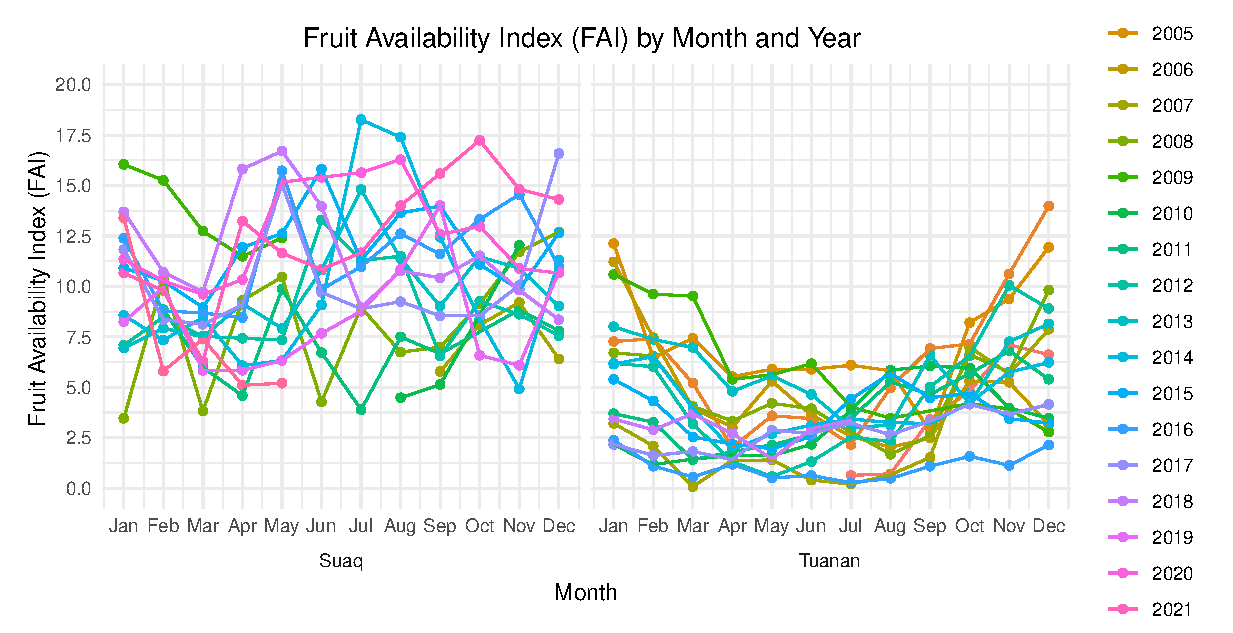
\includegraphics[width=1\linewidth]{Chapter3/Figs/plot.eps}
\caption{Fruit Availability Index (FAI) by month of the year. FAI was calculated as the percentage of trees with fruits across all surveyed trees in the study site. The left plot shows FAI in Suaq (Sumatra), and the right plot shows FAI in Tuanan (Borneo). }
\label{fig:FAI_by_month_between_Suaq_and_Tuanan}
\end{figure}

\subsection{Analysis}

I investigated the impact of the Fruit Availability Index (FAI), study site, and individual orangutans on the relative flange size in orangutans with Gaussian linear mixed-effects models (LMMs) using the \textit{lme4} package in R \citep{Bates.2015}. The model was fit using restricted maximum likelihood (REML), and the significance of the fixed effects was assessed using Satterthwaite's method for approximating degrees of freedom. The model included the fixed effects of: years since first seen, FAI (averaged over three months), study site, and the interactive effect between FAI and study site. Individual orangutan identity was included as a random effect. 

As antagonistic interactions have only been observed in Tuanan, and in absence of a robust proxy, LMMs which examined the impact of antagonistic interactions were only run on the Tuanan measurements. These LMMs included the fixed effects of Years since first seen, FAI (averaged over three months), antagonistic interactions, the interactive effect between antagonistic interactions, and FAI (averaged over three months). Individual orangutan identity was also included as a random effect. 

Null models were created for each model with an effect structure of \(Response ~ 1 + (1|Name)\). All models were run twice, with the response variable being either relative flange width, or relative flange area. Models were evaluated to the null model using Akaike Information Criterion (AIC) with the change in AIC listed next to each model. 

Following the fitting of the models, I examined the normality of residuals and homoscedasticity to validate the model's fit. This was achieved via visual inspection of Q-Q plots and residual versus fitted value plots. Additionally, the variance inflation factor (VIF) was calculated to assess multicollinearity among the predictors. A high VIF for any predictor variable suggests that it is highly collinear with the other predictors, and may necessitate the removal of that variable from the model. 

To assess the potential impact of reduced flange size on mating behaviour and associated long call behaviour, I used Generalized linear mixed models using the \textit{glmTMB} package in R \citep{Brooks.2017}. Continuous response variables, including average duration of long calls and number of hours in association with a female were examined using Gaussian linear mixed-effect models. Count based response variables, including number of long calls per follow day, number of pulses per long call, and number of copulations were assessed with Poission linear mixed-effect models.

All models were tested for over‐dispersion. If data in a model with Poisson distribution revealed over‐dispersion, I conducted negative binomial GLMMs as a robust alternative. All models were created with the nested random intercept of (1|Name/Year/Month), however in the instance of singularity errors, the random intercept was reduced to (1|ID).

All plots were produced using \textit{ggplot2} and \textit{ggeffects} was used to illustrate model effects. All statistical tests are two-tailed unless otherwise stated, and statistical analysis was performed in R version 4.3.0 (\citep{R.2018, Wickham.2011, Lüdecke.2018}. 

\subsection{Ethical note}
Behavioural data collection was strictly observational and non-intrusive. There was no engagement between observers and the wild orangutans; a minimum distance of 10 metres was maintained to ensure the subjects' natural behaviour remained uninfluenced. The procedures for data gathering were in line with Indonesia's legal stipulations and received approvals from the Indonesian State Ministry for Research and Technology (RISTEK), the Directorate General of Natural Resources and Ecosystem Conservation - Ministry of Environment and Forestry of Indonesia (KSDAE-KLHK), the Ministry of Internal Affairs, Indonesia, the Nature Conservation Agency of Central Kalimantan (BKSDA), and the Balai Besar Taman Nasional Gunung Leuser (BBTNGL).

\section{Results}
\subsection{Life history and ecological impacts on relative flange size}
To examine the impact of ecological factors on relative flange size, 8 linear mixed models were fitted by REML using Satterthwaite's method for t-tests. Each model was run twice with the response variable changing between Relative Flange Width and Relative Flange Area. 

Our first pair of models were run on measurements collected from both field sites on the explanatory variables of relative age, the average FAI of the preceding 3 months, field site (as a factor) and an interactive effect between FAI and the field site.

The interaction between zFAI average over three months and study site was not significant (Estimate = 0.046850, p-value = 0.236497), suggesting that the effect of zFAI on relative flange size does not significantly differ between the study sites. As such the model was re-run leaving out this interactive effect.

\begin{table}
    \centering
    \resizebox{\textwidth}{!}{%
    \begin{tabular}{l l r r r r r}
    \hline 
    \multirow{1}{*}{\textit{Response}} & \multirow{1}{*}{\textit{Fixed effects}} & \multirow{1}{*}{\textit{Estimate}} & \multirow{1}{*}{\textit{Std. error}}  & \multirow{1}{*}{\textit{df}} & \multirow{1}{*}{\textit{t-value}}  & \multirow{1}{*}{\textit{p-value}}\\ 
    \hline
   \textbf{1. Proportion of eye flange width} & \textbf{Intercept} & \textbf{1.003} & \textbf{0.039} & \textbf{86.739} & \textbf{25.482} & \textbf{< 0.001}\\

      & \textbf{Years since first seen} & \textbf{-0.009} & \textbf{0.002} & \textbf{43.240} & \textbf{-3.730} & \textbf{0.001}\\

    N = 111, $\Delta$ AIC = 26.19 & zFAI (3 month average) & -0.052 & 0.030 & 99.736 & -1.736 &  0.086\\
 
     & Field Site (Factor) & -0.022 & 0.045 & 78.292 & -0.489 &  0.626\\

    & zFAI (3 month average) : Field site (As factor) & 0.047 & 0.039 & 103.255 & 1.191 &  0.236\\
    \cline{2-7}
        & \textit{Random effects} & & & & \textit{Variance} & \textit{Std. dev.}\\
    \cline{2-7} 
    & Name (Intercept) & & & & 0.002 & 0.043 \\
    & Residual & & & & 0.006 & 0.075 \\
     \hline 
   \textbf{2. Proportion of flange area} & \textbf{Intercept} & \textbf{0.892} & \textbf{0.121} & \textbf{68.527} & \textbf{7.340} & \textbf{< 0.001}\\

     & Years since first seen & -0.005 & 0.007 & 28.726 & -0.702 & 0.488\\

   N = 81, $\Delta$ AIC = 25.846  & zFAI (3 month average) & -0.117 & 0.095 & 73.298 & -1.236 &  0.220\\
 
    & Field Site (Factor) & 0.024 & 0.138 & 67.965 & 0.171 &  0.865\\

    & zFAI (3 month average) : Field site (As factor) & 0.216 & 0.123 & 75.824 & 1.753 &  0.084\\
    \cline{2-7}
        & \textit{Random effects} & & & & \textit{Variance} & \textit{Std. dev.}\\
    \cline{2-7} 
    & Name (Intercept) & & & & 0.009 & 0.092 \\
    & Residual & & & & 0.040 & 0.200 \\
     \hline 
\end{tabular}
    }
    \caption{Results of the LMM examining the impacts of social and ecological factors on the flange size response variables across both field sites.. The fixed effects used were relative age, 3 month average FAI, field site (as a factor) and an interactive effect between 3 month average FAI and field site. This model included a random effect of an individual.
    Formula used was: \(Response \sim YearsSinceFirstSeen + FAI (3MonthAverage) * FieldSite (as.factor) + (1 | Name)\) }
\end{table}
This pair of models showed a significant result. With relative flange width as the response variable (Model 3, Table 3.2), this model revealed a significant effect of years since first seen (relative age) on relative flange width (Estimate = -0.009, p-value < 0.001). 
There was no overall impact of zFAI on relative flange width across sites, nor was a significant difference in flange width observed between the two sites (Estimate = -0.052, p-value = 0.086).

In contrast, where the proportion of flange area was the response variable (Model 4, Table 3.2), I did not find a significant impact of years since first seen on flange size (Estimate = -0.005, p-value = 0.4881). Similar to the all-sites-width model, there was no observed overall relationship between 3 month average FAI and flange size (Estimate = -0.117, p-value = 0.220).

There was no observed significant relationship between field site and relative flange width or area in either model 3 or 4 (Estimate = 0.111, p-value = 0.371; Estimate = 0.024, p-value = 0.865).

\begin{table}
    \centering
    \resizebox{\textwidth}{!}{%
    \begin{tabular}{l l r r r r r}
    \hline 
    \multirow{1}{*}{\textit{Response}} & \multirow{1}{*}{\textit{Fixed effects}} & \multirow{1}{*}{\textit{Estimate}} & \multirow{1}{*}{\textit{Std. error}}  & \multirow{1}{*}{\textit{df}} & \multirow{1}{*}{\textit{t-value}}  & \multirow{1}{*}{\textit{p-value}}\\ 
    \hline
   \textbf{3. Proportion of eye flange width} & \textbf{Intercept} & \textbf{0.990} & \textbf{0.030} & \textbf{71.427} & \textbf{33.086} & \textbf{< 0.001}\\

     & \textbf{Years since first seen} & \textbf{-0.010} & \textbf{0.002} & \textbf{56.544} & \textbf{-4.465} & \textbf{< 0.001}\\

   N = 111, $\Delta$ AIC = 18.371  & zFAI (3 month average) & -0.015 & 0.017 & 113.86 & -0.887 & 0.377\\
 
      & Field Site (Factor) & -0.005 & 0.039 & 81.637 & -0.137 & 0.891\\
    \cline{2-7}
        & \textit{Random effects} & & & & \textit{Variance} & \textit{Std. dev.}\\
    \cline{2-7} 
    & Name (Intercept) & & & & 0.002 & 0.047 \\
    & Residual & & & & 0.005 & 0.074 \\
     \hline 
   \textbf{4. Proportion of flange area} & \textbf{Intercept} & \textbf{0.805} & \textbf{0.098} & \textbf{48.057} & \textbf{8.203} & \textbf{< 0.001}\\

      & Years since first seen & -0.010 & 0.006 & 38.823 & -1.479 & 0.147\\

    N = 81, $\Delta$ AIC = 20.762 & zFAI (3 month average) & 0.036 & 0.054 & 80.933 & 0.668 & 0.506\\
 
    & Field Site (Factor) & 0.111 & 0.124 & 63.613 & 0.900 & 0.371\\

    \cline{2-7}
        & \textit{Random effects} & & & & \textit{Variance} & \textit{Std. dev.}\\
    \cline{2-7} 
    & Name (Intercept) & & & & 0.011 & 0.105 \\
    & Residual & & & & 0.039 & 0.199 \\
     \hline 
\end{tabular}
    }
    \caption{Results of the LMM examining the impacts of social and ecological factors on the flange size response variables across both field sites.. The fixed effects used were relative age, 3 month average FAI, field site (as a factor). This model included a random effect of an individual.
    Formula used was: \(Response \sim YearsSinceFirstSeen + FAI (3MonthAverage) + FieldSite (as.factor) + (1 | Name)\) }
\end{table}

The next pair of models were solely run on the data acquired from Tuanan, which remains the unique site where antagonistic interactions have been directly observed and recorded. The first model (Model 5, Table 3.3) was centred around the proportion of eyeflange with a focus on the potential impacts of antagonistic interactions and the incorporation of an interactive effect between cumulative antagonistic interactions and FAI.

According to this model, no statistically significant impact was found from the hypothesised causes on the proportion of eyeflange (Year since first seen: Estimate = -0.00215, p-value = 0.347; FAI average over three months: Estimate = 0.00273, p-value = 0.750; Cumulative antagonistic interactions: Estimate = -0.00350, p-value = 0.631; FAI average over three months: Cumulative antagonistic interactions: Estimate = 0.00011, p-value = 0.962).

The second model (Model 6, Table 3.3) examined the proportion of flange area. Similar to the first model, it did not find any statistically significant relationship with the hypothesised causes (Year since first seen: Estimate = -0.00186, p-value = 0.754; FAI average over three months: Estimate = 0.02152, p-value = 0.335; Cumulative antagonistic interactions: Estimate = -0.00765, p-value = 0.725; FAI average over three months : Cumulative antagonistic interactions: Estimate = 0.00039, p-value = 0.957).

Since no significant interactive impact between cumulative antagonistic interactions and age or FAI average over three months was found in either of the models, these interactive effects were removed before the models were run again.
\begin{table}
    \centering
    \resizebox{\textwidth}{!}{%
    \begin{tabular}{l l r r r r r}
    \hline 
    \multirow{1}{*}{\textit{Response}} & \multirow{1}{*}{\textit{Fixed effects}} & \multirow{1}{*}{\textit{Estimate}} & \multirow{1}{*}{\textit{Std. error}}  & \multirow{1}{*}{\textit{df}} & \multirow{1}{*}{\textit{t-value}}  & \multirow{1}{*}{\textit{p-value}}\\ 
    \hline
   \textbf{5. Proportion of Eye Flange} & \textbf{Intercept} & \textbf{0.9266} & \textbf{0.0376} & \textbf{64} & \textbf{24.675} & \textbf{< 0.001}\\

      & Years since first seen & -0.0022 & 0.0023 & 64 & -0.947 & 0.347\\

     N = 69, $\Delta$ AIC = 42.73  & FAI (3 month average) & 0.0027 & 0.0085 & 64 & 0.320 &  0.750\\
 
     & Antagonistic cumulative effect & -0.0035 & 0.0073 & 64 & -0.483 &  0.631\\

    & FAI (3 month average) : Antagonistic cumulative effect & 0.00011 & 0.0023 & 64 & 0.048 &  0.962\\
    \cline{2-7}
        & \textit{Random effects} & & & & \textit{Variance} & \textit{Std. dev.}\\
    \cline{2-7} 
    & Name (Intercept) & & & & 0.0000 & 0.000 \\
    & Residual & & & & 0.0064 & 0.080 \\
     \hline 

   \textbf{6. Proportion of Flange Area} & \textbf{Intercept} & \textbf{0.7633} & \textbf{0.0966} & \textbf{50} & \textbf{7.900} & \textbf{< 0.001}\\

      & Years since first seen & -0.0019 & 0.0059 & 50 & -0.315 & 0.754\\

    N = 55, $\Delta$ AIC = 33.71  & FAI (3 month average) & 0.0215 & 0.0221 & 50 & 0.973 &  0.335\\
 
      & Antagonistic cumulative effect & -0.0077 & 0.0216 & 50 & -0.354 &  0.725\\

    & FAI (3 month average) : Antagonistic cumulative effect & 0.00039 & 0.0072 & 50 & 0.054 &  0.957\\
    \cline{2-7}
        & \textit{Random effects} & & & & \textit{Variance} & \textit{Std. dev.}\\
    \cline{2-7} 
    & Name (Intercept) & & & & 0.0000 & 0.000 \\
    & Residual & & & & 0.0345 & 0.186 \\
     \hline 
\end{tabular}
    }
    \caption{Results of the LMM examining the impacts of social and ecological factors on the flange size response variables at the Tuanan field site. The fixed effects used were relative age, 3 month average FAI, cumulative antagonistic interactions and an interactive effect between 3 month average FAI and cumulative antagonistic interactions. This model included a random effect of an individual. 
    Formula used was: \(Response \sim YearsSinceFirstSeen + FAI (3MonthAverage) * CumulativeAntagonisticInteractions + (1 | Name)\) }
\end{table}


The final pair of models, which were run only on the Tuanan site, included cumulative antagonistic interactions, but without the interactive effect between antagonistic interactions and zFAI (Table 3.4). When the response variable was proportion of flange area (Model 7, Table 3.4), I did not find any significant impact from any of the hypothesised factors. Likewise, when the response variable was proportion of eye flange (Model 8, Table 3.4), again, no significant impact was found from any of the factors. 

\begin{table}
    \centering
    \resizebox{\textwidth}{!}{%
    \begin{tabular}{l l r r r r r}
    \hline 
    \multirow{1}{*}{\textit{Response}} & \multirow{1}{*}{\textit{Fixed effects}} & \multirow{1}{*}{\textit{Estimate}} & \multirow{1}{*}{\textit{Std. error}}  & \multirow{1}{*}{\textit{df}} & \multirow{1}{*}{\textit{t-value}}  & \multirow{1}{*}{\textit{p-value}}\\ 
    \hline
   \textbf{7. Proportion of eye flange} & \textbf{Intercept} & \textbf{0.926} & \textbf{0.032} & \textbf{65} & \textbf{29.039} & \textbf{< 0.001}\\

     & Years since first seen & -0.00215 & 0.00225 & 65 & -0.953 & 0.344\\

    N = 69, $\Delta$ AIC = 31.59  & FAI (3 month average) & 0.00302 & 0.00599 & 65 & 0.503 & 0.616\\
 
    & Antagonistic cumulative & -0.00319 & 0.00305 & 65 & -1.045 & 0.300\\
    \cline{2-7}
        & \textit{Random effects} & & & & \textit{Variance} & \textit{Std. dev.}\\
    \cline{2-7} 
    & Name (Intercept) & & & & 0.00000 & 0.000 \\
    & Residual & & & & 0.006345 & 0.080 \\
    \hline
   \textbf{8. Proportion of flange area} & \textbf{Intercept} & \textbf{0.760} & \textbf{0.081} & \textbf{51} & \textbf{9.417} & \textbf{< 0.001}\\

      & Years since first seen & -0.00182 & 0.00579 & 51 & -0.314 & 0.755\\

    N = 55, $\Delta$ AIC = 25.13  & FAI (3 month average) & 0.02237 & 0.01548 & 51 & 1.445 & 0.154\\
 
     & Antagonistic cumulative & -0.00660 & 0.00896 & 51 & -0.736 & 0.465\\
    \cline{2-7}
        & \textit{Random effects} & & & & \textit{Variance} & \textit{Std. dev.}\\
    \cline{2-7} 
    & Name (Intercept) & & & & 0.00000 & 0.000 \\
    & Residual & & & & 0.03383 & 0.184 \\
     \hline 
\end{tabular}
    }
    \caption{Results of the LMMs examining the impacts of social and ecological factors on the flange size response variables at the Tuanan field site. The fixed effects used were relative age, 3 month average FAI, cumulative antagonistic interactions. This model included a random effect of an individual. 
    Formula used was: \(Response \sim YearsSinceFirstSeen + FAI (3MonthAverage) + CumulativeAntagonisticInteractions + (1 | Name)\) }
\end{table}


\begin{figure}
\centering
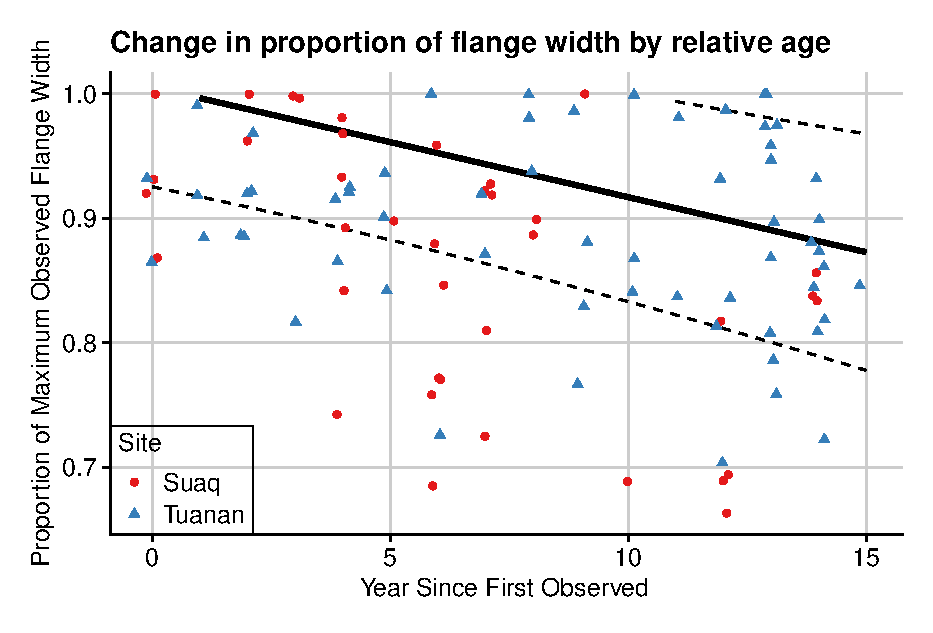
\includegraphics[width=0.8\linewidth]{Chapter3/Figs/flange_width.eps}
\caption{Examination of the impacts of ecological and social factors on flange width in orangutans across different sites. The plot presents the relationship between the number of years since the orangutan was first observed (YearSinceFirstSeenTab) and the proportion of maximum observed flange width (Prop\_eyeflange). Each point, differentiated by colour and shape according to the site, represents an observation from the data set. The lines with dashed boundaries show the predicted response and confidence intervals generated from the mixed model results.}
\label{fig:enter-label}
\end{figure}
\subsection{Impacts of relative flange size on long calls and mating success}

In the analysis of the effect of relative flange width on flanged male mating behaviour, five models were considered. Table 3.5. shows Models 9-11, based on count data.

Model 9 (Table 3.5.), focused on the number of long calls per follow day, found a statistically significant impact of relative flange width on the number of long calls produced per day (Estimate = -7.697, p-value = 0.034). Additionally, I found a significant impact of the total hours of rainfall per follow day on long call rates, albeit with a lower effect size (Estimate = 0.076, p-value = 0.025). However, no other explanatory variable was found to be significant.

 Model 10, which considered the number of pulses per long call per follow day, did not reveal significant impacts from any of the variables, except Total rain (hours) which showed a minor positive impact on the number of pulses per long call (Estimate = 0.011, p-value = 0.027).
 
Model 11, analysing the number of copulations per follow day, did not find any significant impacts between the proposed factors and the number of copulations per follow day. 

\begin{table}
    \centering
    \resizebox{\textwidth}{!}{%
    \begin{tabular}{l l r r r r}
    \hline 
    \multirow{2}{*}{\textit{Response}} &  \multirow{2}{*}{\textit{Fixed effects}} & \multirow{2}{*}{\textit{Estimate}} & \multirow{2}{*}{\textit{Std. Error}} & \multirow{2}{*}{\textit{z}} & \multirow{2}{*}{\textit{Pr(>|z|)}}\\ 
     & & & & & \\
    \hline
   \textbf{9. Number of long calls per follow day} & \textbf{Intercept} & \textbf{-2.632} & \textbf{3.278} & \textbf{-0.803} & \textbf{0.422} \\

   & \textbf{Prop\_eyeflange }& \textbf{-7.697} & \textbf{3.631} & \textbf{-2.120} & \textbf{0.034} \\
   
   \textit{Negaitve Binomial GLMM} & zFAI & 0.904 & 0.727 & 1.244 & 0.214\\
   
   \textit{Offset(ObsTime)} & Site (Tuanan) & 0.742 & 1.700 & 0.437 & 0.662\\
    
   N = 75, $\Delta$ AIC = 25.13 & \textbf{Long calls heard} & \textbf{0.231} & \textbf{0.118} & \textbf{1.965} & \textbf{0.049} \\
   
   & zAssocH & -0.091 & 0.275 & -0.331 & 0.741\\
   
   & \textbf{Total rain (hours)} & \textbf{0.076} & \textbf{0.034} & \textbf{2.237} & \textbf{0.025}\\
   
    \cline{2-6}
    
        & \textit{Random effects} & & & \textit{Variance} & \textit{Std. dev.}\\
        
    \cline{2-6} 
    
    & Name & & & 1.012e-09 & 3.181e-05 \\

    & Year:Name & & & 4.974 & 2.230 \\
    
    & Month:Year:Name & & & 5.625e-08 & 2.372e-04 \\
    
     \hline 

   \textbf{10. Number of pulses per long call} & \textbf{Intercept} & \textbf{2.477} & \textbf{0.934} & \textbf{2.654} & \textbf{0.008} \\

  & Prop\_eyeflange & 0.812 & 1.093 & 0.743 & 0.458 \\
   
   & zFAI & -0.055 & 0.204 & -0.271 & 0.787\\
   
    \textit{Negaitve Binomial GLMM} & Site (Tuanan) & -0.253 & 0.557 & -0.454 & 0.650\\
    
  & Long calls heard & 0.020 & 0.019 & 1.085 & 0.278 \\
   
 N = 29, $\Delta$ AIC = 2.034  & zAssocH & -0.052 & 0.061 & -0.851 & 0.395\\
   
   & \textbf{Total rain (hours)} & \textbf{0.011} & \textbf{0.005} & \textbf{2.212} & \textbf{0.027}\\
   
    \cline{2-6}
    
        & \textit{Random effects} & & & \textit{Variance} & \textit{Std. dev.}\\
        
    \cline{2-6} 
    
    & Name & & & 0.208 & 0.456 \\

     \hline 
   \textbf{11. Number of copulations per follow day} & \textbf{Intercept} & \textbf{-15.440} & \textbf{65.063} & \textbf{-0.237} & \textbf{0.812} \\

   & Prop\_eyeflange & -4.302 & 68.047 & -0.063 & 0.950 \\
   
   \textit{Poisson GLMM}, \textit{N = 23} & zFAI & -0.718 & 4.399 & -0.163 & 0.870\\
   
  \textit{Offset(FemAssocH)}  & Site (Tuanan) & -2.444 & 9.599 & -0.255 & 0.799\\
    
  N = 23, $\Delta$ AIC = 13.04  & Long calls made & 0.430 & 1.009 & 0.426 & 0.670 \\
      
    \cline{2-6}
    
        & \textit{Random effects} & & & \textit{Variance} & \textit{Std. dev.}\\
        
    \cline{2-6} 
    
 & Name & & & 8.494e-04 & 0.029 \\

    & Year:Name & & & 0.001 & 0.037 \\
    
    & Month:Year:Name & & & 76.10 & 8.723 \\
    
     \hline 
       \end{tabular}
}
    \caption{Results of the GLMMs exploring the impacts of relative flange width and ecological factors on number of long calls per follow day, number of pulses per long call and number of copulations.}
\end{table}
Table 3.6. shows Models 12-13, which are both based on continuous response variables. In Model 12, the response variable was the "Average duration of long call per follow day". None of the fixed effects demonstrated a significant impact on the duration of long call per follow day.  Model 13 aimed to understand the impact of these fixed effects on the number of hours in association with a female per follow day. Notably, zFAI demonstrated a significant impact, with an estimate of -1.30278 and a p-value of 0.048. However none of the other explantory variables showed a statistically significant impact.

\begin{table}
    \centering
    \resizebox{\textwidth}{!}{%
    \begin{tabular}{l l r r r r r}
    \hline 
    \multirow{2}{*}{\textit{Response}} &  \multirow{2}{*}{\textit{Fixed effects}} & \multirow{2}{*}{\textit{Estimate}} & \multirow{2}{*}{\textit{Std. Error}} & \multirow{2}{*}{\textit{df}} & \multirow{2}{*}{\textit{t}} & \multirow{2}{*}{\textit{Pr(>|t|)}}\\ 
     & & & & & & \\
    \hline
        \textbf{12. Average duration of long call per} & Intercept & 95.85126 & 60.62015 & 18 & 1.581 & 0.131 \\

  \textbf{follow day} & Prop\_eyeflange & -44.87252 & 70.46522 & 18 & -0.637 & 0.532 \\
   
   & zFAI & -1.78435 & 12.52036 & 18 & -0.143 & 0.888\\
   
    \textit{Gaussian GLMM}, \textit{N = 25} & Site (Tuanan) & -17.13861 & 25.83756 & 18 & -0.663 & 0.516\\
    
    & zAssocH & -0.14225 & 4.89118 & 18 & -0.029 & 0.977 \\
   
  N = 25, $\Delta$ AIC = 36.71 & LCH & 0.53515 & 1.37842 & 18 & 0.388 & 0.702\\
   
   & Total rain (hours) & 0.01575 & 0.37449 & 18 & 0.042 & 0.967\\
   
    \cline{2-7}
    
        & \textit{Random effects} & & & & \textit{Variance} & \textit{Std. dev.}\\
        
    \cline{2-7} 
    
    & Name & & & & 0 & 0 \\

    & Residual & & & & 541.7 & 23.28 \\
    
     \hline 

        \textbf{13. Number of hours in association} & Intercept & -1.40594 & 0.94322 & 74.30810 & -1.491 & 0.1403 \\

  \textbf{with a female per follow day} & Prop\_eyeflange & 1.52725 & 1.02205 & 86.91673 & 1.494 & 0.1387 \\
   
   & \textbf{zFAI} & \textbf{-0.19514} & \textbf{0.09292} & \textbf{96.48181} & \textbf{-2.100} & \textbf{0.0383}\\
   
    \textit{Guassian GLMM} & Site (Tuanan) & -0.15691 & 0.20012 & 25.63337 & -0.784 & 0.4402\\
    
\textit{Offset(ObsTime)}  & Long calls made & 0.04682 & 0.02471 & 94.76339 & 1.895 & 0.0611 \\
   
   
    \cline{2-7}
    
      N = 119, $\Delta$ AIC = 25.11  & \textit{Random effects} & & & & \textit{Variance} & \textit{Std. dev.}\\
        
    \cline{2-7} 
    
    & Name & & & & 0.01186 & 0.1089 \\

    & Year:Name & & & & 0.08261 & 0.2874 \\
    
    & Month:Year:Name & &&  &  0.00000 &  0.0000 \\

    & Residual & & & & 0.88910 & 0.9429 \\
    
     \hline 

    \end{tabular}
    }
    \caption{Results of the LMMs examining the impacts of relative flange width on average duration of long call and number of hours of female association per follow day. }
\end{table}



\section{Discussion}

The maintenance of SSCs can be metabolically costly for the individuals who produce them, however their ultimate impact on mating success depends on the mating system, dominance hierarchy and life history of the species \citep{Kappeler.2004}. 

\subsection{Impact of life history and ecological factors on flange size}
Our model which examined the hypothesised causes of flange reduction across all sites indicated that age was the best linear predictor of reduction in flange width (although this was not found to be significant in the Tuanan-only models, or on relative flange area). This is particularly notable as it suggests that the cause is likely not accumulated injuries and scar tissue on the flange, as these injuries can occur all over the flange rather than localised at the eye level. As these impacts were only seen in one model with a limited sample size, it is important not to overstate their significance, however they may be indicative of age related degeneration in the flange. Older individuals experience senescence, which may have several impacts on SSC maintenance. I suggest four non-mutually exclusive mechanisms for degeneration in flange size after initial development.

The first is age-linked reduction in testes volume, which in turn has an impact on circulating testosterone levels. In humans, males over the age of 60 experience a reduction in testes size of approximately 37\%, and mean serum testosterone levels start decreasing from the age of 50 \citep{Stearns.1974}. Across wild and captive studies, flanged males have significantly higher androgen levels than unflanged males, and individuals undergoing bimaturism have higher levels still indicating their importance to the development and maintenance of these characteristics \citep{Marty.2015rzq, Prasetyo.2021}. Hence an age-linked reduction in testosterone due to age may impact the maintenance of these SSCs. 

A second possible cause of a reduction in flange width with old age is sarcopenia, the deterioration of muscle tissue in elderly mammals. This progressive and generalised skeletal muscle disorder involves the accelerated loss of muscle mass and function \citep{Evans.1993}. In the case of the orangutan flange, which houses slips of several of the facial muscles \citep{Straus.1942}, such age-related muscle wasting could be particularly impactful. The loss of these muscle fibres might directly translate to a decrease in the structural support required for maintaining flange size, thereby leading to a decrease in the mass and volume of the flanges.

A third potential mechanism behind the age-related reduction in flange size may be tied to reduced vascularity associated with aging. The process of aging is linked to the diminished vascular supply of tissues, thereby limiting the amount of oxygen and nutrients delivered to these tissues, and subsequently impeding their repair and regeneration capabilities \citep{Prisby.2007}. Dissections of the orangutan flange, the skin and the underlying fatty pad appear to be quite vascular \citep{Straus.1942}. These regions are abundant with blood vessels, with some areas suggestive of erectile tissue due to the density of vasculature. Given this, the flanges might be particularly vulnerable to the effects of reduced vascularity that come with aging. The reduction in blood supply could deprive the fibrous and adipose tissues, which make up the bulk of the flange, of the necessary resources for maintenance and repair.
In the face of diminished vascularity, the fibrous framework consisting of collagenous septa, along with the lobules of fat and striated muscle fibres found in the flange \citep{Straus.1942, Winkler.1989}, might experience reduced nutritional and oxygen supply. This could potentially lead to a decrease in the integrity and mass of these components, subsequently contributing to a reduction in flange size. Hence, this relationship between reduced vascularity and the age-related decrease in flange size may serve as a compelling avenue for future research.

Finally, the structural integrity of flanges, which are largely composed of loose connective tissue whose framework consists of collagenous septa continuous with the fibres of the corium, might be impacted by age-related collagen deterioration \citep{Straus.1942}. As aging progresses, there is a decline in collagen synthesis, coupled with a slowing of the tissue remodelling process. This could lead to a decreased structural integrity of the collagenous framework of the flanges, rendering them less robust and potentially smaller. The accumulation of damage, as a result of less efficient tissue repair and replacement, could further contribute to the degradation of fibrous tissues in the flanges \citep{Cox.2011, Haus.2007}. As previously mentioned, these hypotheses are not mutually exclusive and these factors may act in synergy.

\subsection{Impact of FAI on flange morphology}

Contrary to my predictions, there was no significant impact of fruit availability on flange size. While the flange structure in orangutans does contain large lobules of fat, this adipose tissue might not be as responsive to changes in nutritional availability as those in other parts of the body. 

It is possible that once flanges have developed, they may not be subject to the same plasticity seen in other phenotypic traits. The flanges, consisting of collagenous septa, striated muscle fibres, and a dense network of blood vessels within a framework of adipose tissue \citep{Straus.1942, Kinglsey.1988} could be resistant to fluctuations in size due to environmental conditions. The high energetic cost associated with flange formation might make it metabolically impractical for the body to adjust these structures in response to varying fruit availability. In fact, this pattern aligns with what has been observed in other primates, such as gorillas, where the size of secondary sexual characteristics like the sagittal crest, remain largely unchanged after full development, despite variations in food availability \citep{Caillaud.2008m5r}.

Second, changes in fruit availability may affect aspects of the flanges other than their width or overall size. For example, reduced availability of nutrients could potentially impact the vascular integrity of the flanges or the health of the dermal papillae. The impact might be seen in visual changes, such as the reported deflated appearance associated with the "past-prime" condition, which could influence the male's attractiveness or social status without altering the overall width of the flanges. Further investigation is required to explore these possibilities and to gain a better understanding of how ecological variables such as fruit availability may impact the physiological characteristics of orangutan flanges using qualitative methodology, or dissection of flange specimens from a range of adults. Notably, a reduction in the volume of the flange that does not impact the area or width would not have been detected by my analyses, however detecting this change in future studies would likely prove difficult, as it would require detailed measurements of the flange in an environment where nutritional intake could be controlled in an manner consistent with animal welfare.

\subsection{Impact of observed antagonistic interactions}
Despite initial conjectures, my analyses focused on the Tuanan field station have found no observed relationship between relative flange size and the frequency or severity of antagonistic interactions. It was previously hypothesised that, due to repeated activation of the vertebrate stress response increasing allostatic loads, flange deformation might be linked to such antagonistic interactions. Across primate species, stress induced by these interactions is well documented to increase blood glucocorticoid concentrations via the activation of the hypothalamus–pituitary–adrenal axis \citep{Maestripieri.2011, Setchell.2016, Edes.2017}.

For example, in mandrills, chronic activation of the vertebrate stress response leads to persistently elevated blood glucocorticoid levels, negatively impacting individual outcomes, including reduced resistance to disease and compromised reproductive success \citep{Setchell.2010}. However, the impacts of stress are modulated by factors such as the individual's dominance ranking and the stability of the dominance hierarchy within the population. The Tuanan field station is characterised by an unstable dominance hierarchy, which is influenced by a high ratio of flanged to unflanged males and significant fluctuations in fruit production. Consequently, I had predicted that the dominant flanged males would experience the greatest social stress during antagonistic interactions \citep{Sapolsky.2005gvn}.

However, a key limitation of this study was the uniform scoring assigned to all antagonistic interactions, regardless of their severity, ranging from immediate withdrawal from the conflict to lethal aggression \citep{Knott.2008, Setia.2008}. Frequently witnessed consequences of these conflicts are mutilations, including loss of digits or bites that remove parts of the upper lip. If these injuries could be reliably dated to specific time frames, they could yield valuable insights for future research into the relationship between social stressors and physical alterations in orangutans. Nonetheless, the current methodology may have obscured potential impacts of the severity of antagonistic interactions on flange morphology, which presents an area for refinement in future studies.

\subsection{Impacts of flange deformation on long call behaviour}

Contrary to my predictions, individuals with a relatively less wide flange produced long calls more often than when their flange was at its fullest extent. Additionally, the total amount of rain hours in the day appears to increase the number of long calls produced, rather than decreasing it - contrary to the findings of previous studies \citep{Spillmann.2016}

One potential explanation for less wide flanged males producing more long calls might lie in their need for enhanced social communication. Orangutans whose flanges are relatively reduced may be lower in the local dominance hierarchy. These individuals might employ long calls more frequently as a strategic tool to communicate their presence, assert their territory, or possibly attract potential mates without engaging in direct physical confrontations, which they are less likely to win due to their less intimidating physicality. These results may also support the hypothesis from \citet{Mitani.1985}, that the flange also functions as a way of focusing the long call in a specific direction. If this hypothesis is correct, then individuals with relatively diminished flange size may need to produce long calls more often to counter the impacts of this condition.

Regarding the increase in the number of long calls with more rain hours, this might be tied to the acoustic properties of the rainforest environment during and after rainfall. It is possible that the ambient noise caused by rainfall masks the long calls, necessitating more frequent vocalisations and an increased number of pulses per vocalisation for effective signaling \citep{Spillmann.2016}. Additionally, during a downpour, the ambient noise levels in the rainforest drop significantly, which may be due in part to the physical impact on the vegetation. It can weigh down foliage, leading to fewer leaves rustling in the wind and therefore less background noise. However, gibbons vocalise less frequently after rainfall, and this quieter backdrop might enhance the audibility of orangutan long calls \citep{Clink.2020}. 

This study did not have access to the raw long call recordings and, as such, I was unable to examine any correlation between other aspects of the long call, including frequency or estimated amplitude with changes in flange width. As long call data sets increase with time, this may be an avenue of research in the future, however, currently long call recordings at Suaq Balimbing and Tuanan are not common enough, or collected over a long enough time to provide a rigorous analysis of longitudinal changes in long call frequency or amplitude.

\subsection{Impacts of flange deformation on female association patterns}

The absence of a direct relationship between flange width and the z-transformed hours of female association per follow day was contrary to my initial hypothesis. I had anticipated that a decrease in flange size would correspond with reduced association hours, under the assumption that physical characteristics such as flange size may be an important factor in female mate choice. However, the lack of evidence for this relationship in the model suggests that flange width might not be as influential a factor as I had initially proposed.

Interestingly, the results did indicate a significant relationship between z-transformed fruit availability and hours of female association, but in a direction opposite to what I had predicted. This counter-intuitive outcome implies that higher fruit availability corresponded with reduced hours of association with females.

One possible explanation for these observations could be that the females are using additional signals beyond their physical characteristics when associating with potential mates. For example, behavioural traits, such as aggressiveness or protectiveness, might be more important determinants of association patterns than physical traits like flange width. Alternatively, it is possible that the significance of flange size is obscured by other unmeasured factors that also affect female association patterns, including familiarity with the flanged male.

Regarding the unexpected inverse relationship between fruit availability and hours of female association, one possible hypothesis could be that when food is plentiful, females may be less dependent on males for resource access and hence spend less time in association. Alternatively, higher fruit availability could result in a more dispersed distribution of individuals within the population, thereby reducing the opportunity for association.

Future research will be needed to test these hypotheses and elucidate the complex interplay of factors affecting association patterns in the study population. Additionally, it would be interesting to investigate the potential role of other male physical and behavioural traits in female association patterns to gain a more nuanced understanding of mate selection processes in this species.

\subsection{Copulation rates}

Contrary to my initial expectations, the number of copulations per follow day did not decline with a decrease in the flange size. The absence of a significant association suggests that flange quality is not a determinate factor when a female is already in association with a male. This may suggest that there is a role of female choice before entering into an association with a male, likely when hearing a long call. However, in this study, I did not find an expected significant association between long calls made and total female association hours per follow day (Model 13). It is plausible that females are more inclined to prioritise other aspects of male behaviour, such as feeding tolerance or food sharing, when selecting mates. Consequently, these behavioural traits could be more strongly tied to reproductive success than flange size. Also to consider is the impact of forced copulations, as this study did not have sufficient data between proceptive and forced copulations this may mask the role of female choice when in association, which led to no detectable significant relationship. 

Similarly, the lack of a significant relationship between relative fruit availability (zFAI) and the number of copulations suggests that immediate ecological conditions, such as food availability, may not directly influence mating behaviours, despite previous studies indicating that they increase association rates \citep{Marshall.2008}. This points towards the possibility that mating activities in this species could be less susceptible to fluctuating resource availability than initially assumed.

However, it is crucial to interpret these findings with caution due to the relatively small sample size of this study. The low number of observations could limit the robustness of the findings and potentially mask existing relationships. A wider comparison between sites in future studies could provide a more reliable analysis of the interaction between relative flange size, mating behaviours, and ecological conditions.

\subsection{Questions not addressed}

One limitation of this study was the inability to examine the impacts of antagonistic social stress at Suaq Balimbing. Face-to-face antagonistic interactions between flanged males have never been observed at Suaq Balimbing, despite having the highest density of wild orangutans in the world. However, orangutans do utilise long calls as a form of confrontational assessment, and this has been used in some studies to estimate dominance, but due to the complexities of this analysis this was beyond the scope of this study \citep{Spillmann.2016}

Another unknown from this research is the correlation between the ecological, social and individual factors and the underlying hormonal processes that drive SSC development and maintenance. While hormonal impacts on flange development have been examined in captivity, the difficulties in obtaining and processing wild hormone samples have made a comprehensive study of the maintenance of these SSCs impractical at this stage.

Due to the suggested relationship between age and relative flange width, and in light of the limited sample size, further studies should seek to examine the relationship between age and mating behaviours in orangutans to examine correlations between age and deterioration of other SSCs (e.g. long call composition and duration) (see Chapter 4).

Finally, in this analysis, individual measures were pooled to assess overall patterns and trends. However, a more granular analysis within-subject vs. between-subjects could offer different insights \citep{Siracusa.2022}. This approach may be able to discern individual trajectories and pinpoint variations that may be unique to specific subjects. Although time constraints prevented the incorporation of this approach into the present study, it represents a promising avenue for future investigations. 

\nomenclature[z-SSC]{SSC}{Secondary Sexual Characteristic}
\nomenclature[z-LM]{LM}{Landmark}
\nomenclature[z-FAI]{FAI}{Fruit Availability Index}
